\section{RESULTS}
We refer to \cite[Ch. 9]{robinson2004simulation}. The system in consideration has a fixed schedule since they open every business day at 6 a.m. and closes at 7 p.m. (Saturdays from 7 a.m. to 1 p.m.), therefore it can be considered as a terminating simulation model. Consequently, the output of the simulation is transient, hence the distribution of the output is constantly changing. For instance, the number of patients is not the same for each day.

The initial condition is assumed as zero because the system does not start with patients inside of it, although, in the complex, patients start arriving before the opening hour and start accumulating. Therefore, it is clear that the distributions in the first hour for all days are biased and this issue cannot be addressed with the available data.

How many times do we have to run the model in order to obtain trustworthy results? When the model is being simulated, it is desired to obtain the highest achievable accuracy, but this often requires a lot of simulation runs and, therefore, computational resources and time. Given that these objectives are conflictive, the idea is to find a balance between them. To achieve this goal, we use the strategy proposed in \cite{byrne2013many} and \cite{currie2016practical}.

This methodology is based on confidence intervals; we select a maximum allowed deviation $\delta$, in terms of a proportion of the mean. The simulation has to be previously run $n_0$ times, to estimate the standard deviation. The appropriate number must satisfy 

\begin{equation}
n \geq\left(\frac{t_{\alpha/2;n_0-1} \times \sigma}{\delta}\right)^{2}
\end{equation} 

Calculating this value for our model, using the test described previously we obtain a large value of $n$. The reason for this is because the fit distributions can generate a big amount of outliers, therefore it is difficult to find stability for the means.

Figure \ref{fig:time_series} is a time series of the average waiting time of the model for a trial of 5 weeks, which shows clearly that the nature of the output is transient since it changes constantly.

\begin{figure}[H]
    \centering
    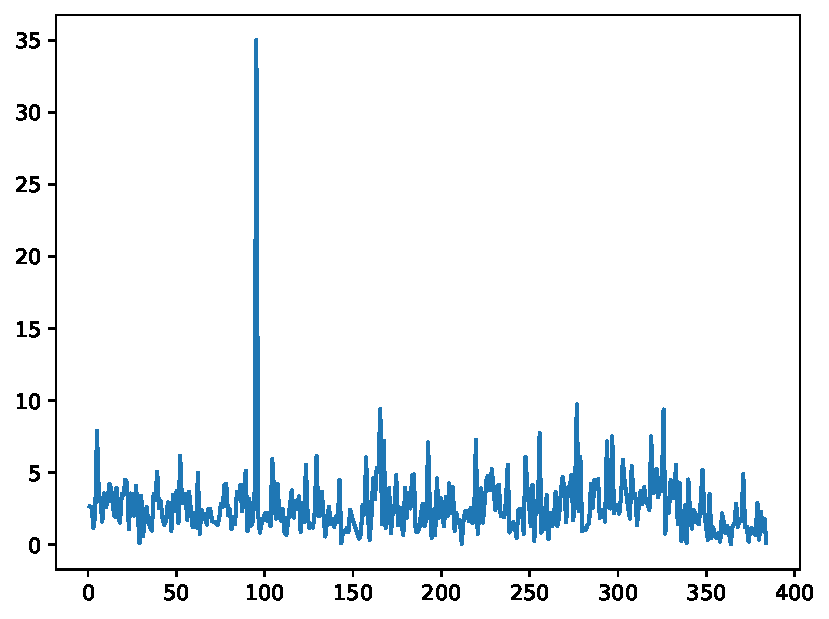
\includegraphics[scale=0.5]{time-series.pdf}
    \caption{Time series for average waiting time in a week}
    \label{fig:time_series}
\end{figure}
